\documentclass[12pt,letterpaper,titlepage]{article}
%\usepackage[latin1]{inputenc}
\usepackage[spanish]{babel}


\usepackage[utf8]{inputenc}
\usepackage{ragged2e}
\usepackage{amsmath}
\usepackage{amsfonts}
\usepackage{amssymb}
\usepackage[none]{hyphenat}
\tolerance =3000
\pretolerance =2000

\usepackage[bookmarks]{hyperref}%,colorlinks,citecolor=black,linkcolor=black,urlcolor=black
\usepackage{appendix}
\usepackage{multirow}
\usepackage{graphicx}
%Modificar margenes
\usepackage{anysize}

%\usepackage{fancyBOX}

%Para crear el encabezado y pie de pagina a nuestro gusto
\usepackage{fancyhdr}

% TABLA
\usepackage{dcolumn}
\usepackage{multirow}
\usepackage{slashbox}
\usepackage{rotating}
\usepackage{graphicx}

%COLOR
\usepackage{colortbl}

%Creamos el encabezado y pie de pagina
\pagestyle{fancy}
\fancyhf{}%Borra todas las configuraciones
\fancyhead[L]{\footnotesize \leftmark}%Alineado a la izquierda CAPITULO # %TITULO DE %CAPITULO
\fancyhead[R]{\footnotesize \thepage}%Alineado a la derecha numero de pagina
\fancyfoot[C]{\footnotesize \thepage}%Centrado numero de pagina
\renewcommand{\headrulewidth}{0.4pt}
\setlength{\headheight}{13pt}%Aumentamos el tama\~no del contenedor para el %encabezado

%Margenes izquierdo - derecho - superior - inferior
\marginsize{3cm}{2.5cm}{2.5cm}{2.5cm}
\author{Francisco Argüelles Granados}
\title{Estado del Arte}
\date{\today}
%%%%%%%%%%%%%%%%%%%%%%%%%%%%%%%% BEGIN DOCUMENT
\begin{document}

\textbf{}
%\maketitle
%\linebreak 
%\linebreak 
%\linebreak 
%
%\begin{center}
%\textit{Diseño de una plataforma web para el análisis de 
%cromosomas enfocado a la toma de decisiones.}
%\end{center}

%\newpage
\setlength{\unitlength}{1 cm} %Especificar unidad de trabajo
\thispagestyle{empty}
\begin{picture}(4,4)
\put(4.3,0){
\includegraphics[width=5cm,height=4cm]{itcv.jpg}}
\end{picture}
\\
\begin{center}
\textbf{{\Huge Instituto Tecnológico de Ciudad Victoria}\\[0.5cm]
{\large Maestría Profesionalizante en Sistemas Computacionales}}\\[1cm]
{\Large Protocolo de tesis}\\[1.3cm]
{\LARGE \textbf{Diseño de una plataforma web para el análisis de 
cromosomas enfocado a la toma de decisiones}}\\[1.5cm]
{\large Francisco Argüelles Granados}\\[1cm]
\textbf{Asesor de Tesis:}\\
Dr. Pedro Sánchez Orellana\\[0.7cm]
%{\large Beca:DGEST }\\[0.7cm]
Ciudad Victoria, Tamaulipas -  \today\

\end{center}


%%%%%%%%%%%
\newpage
\begin{center}
\tableofcontents
\end{center}
\newpage
\glossary{Resumen}
\section{Resumen}\label{resumen}


%En el mundo actual existen una gran cantidad de aplicaciones enfocadas a la generación de información misma que bombardea a usuarios con datos no necesariamente relevantes, pues dichas aplicaciones presentan puntos de opinión sin tener fundamentos sustentables como investigaciones o referencias bibliográficas de índole científica o tecnológica. 

%Esta problemática se presenta en diferentes nichos, por ejemplo, en el caso del sector salud el uso de imágenes de laboratorio facilita el diagnóstico temprano de malformaciones congénitas. Sin embargo, la interpretación de la información no es una tarea sencilla, pues se requiere realizar una serie de pasos para llegar a un diagnóstico satisfactorio. Otro ejemplo es el caso del análisis de los patrones de expresión en el rostro y cuerpo, empleados durante los test psicométricos o en evaluaciones psiquiátricas. Si bien es cierto que éstos pueden ser valorados por un especialista en el área, dichas valoraciones carecen de una métrica general independiente a la perspectiva del especialista. 

%En ambos casos los problemas mencionados, actualmente se poseen metodologías y técnicas que facilitan la extracción de la información; sin embargo, no así el análisis de los datos proporcionados. Es en este punto donde los modelos computacionales juegan un papel relevante pues permiten establecer patrones y relaciones de la información obtenida. De forma más específica, los modelos computacionales enfocados a la web facilitan el acceso y uso de dichas herramientas de análisis a un gran número de personas distribuidas en diferentes puntos geográficos.

%\begin{quotation}
Nuestro mundo actual esta prominentemente dominado por la tecnología, vivimos en una sociedad donde los avances tecnológicos son parte de nuestra vida diaria y muchas veces dependemos de ellos para poder llevar a cabo nuestras actividades cotidianas.\\

%\end{quotation}
%\begin{quotation}
Muchos avances tecnológicos ha venido a ayudar a otras áreas como la Economía y el Arte, por mencionar a algunas, y sin lugar a dudas el Sector Salud ha sido también beneficiado con diversos equipos tecnológicos que sirven de apoyo al servicio de salubridad, tanto a nivel local, nacional y mundial.\\

%\end{quotation}
%\begin{quotation}
Aún y cuando esta tecnología nos ayuda a proporcionar servicios para atención y prevención de enfermedades hereditarias, los equipos diseñados con este fin son demasiado caros y pocos son los hospitales y centros de salud que los poseen y cuentan con personal calificado para su operación, lo que ocasiona que el servicio de cariotipo -que es el atañe a esta propuesta de tesis- tiene un costo caro y que para algunas personas no es tan fácil poderlo realizar, como por ejemplo a la población que habita en zonas rurales no le es tan fácil desplazarse a las grandes ciudades donde por lo regular se realiza este tipo de estudio.\\
%\end{quotation}
Es aquí donde se pretende aprovechar los avances tecnológicos, principalmente el uso de Internet donde se puede tener acceso en la mayor parte del país incluyendo las zonas rurales. Esto con el fin poder establecer un Servicio Web que permita realizar el cariotipo y generar un reporte que apoye al diagnóstico del médico en cuestión.\\

%%%%%%%%%%%%%%%%%%%%%%% INTRODUCCION
%\newpage
%\glossary{Introduccion}
\section{Introducción}\label{intro}
%\begin{quotation}
La presente propuesta de tesis está enfocada a proporcionar una herramienta computacional enfocada a la toma de decisiones en el sector salud. De manera más específica, en el rubro de diagnóstico de laboratorio e imagenología. El producto que se espera obtener es un servicio web auxiliar en el diagnóstico temprano de enfermedades genéticas. El cariotipo es un esquema o imagen de los cromosomas de una célula metafásica ordenados de acuerdo a su morfología y tamaño. Mediante el proceso de cariotipado se pueden analizar diversas anomalías cromosómicas. En el Hospital Infantil de Tamaulipas (HIT) se ha utilizado dicho proceso para detectar algunas anomalías cromosómicas como el Síndrome de Turner, de Klinefelter, de Betwith-Wiedeman, de Down y de Prader Willi. Todos estos síndromes son altamente discapacitantes y reducen la calidad y el tiempo de vida de las personas afectadas. \\
%\end{quotation}

%\begin{quotation}
Estos análisis cromosómicos se realizan a partir de una muestra de sangre o de tejido. Para poder observar los cromosomas con un microscopio, la muestra debe ser teñida y fotografiada. A partir de esa fotografía, un experto puede separar y organizar los cromosomas de acuerdo a su forma y tamaño. Esta tarea requiere de varios días para ser completada. Debido a la gran cantidad de tiempo que implica la realización de este estudio, algunas compañías han comercializado herramientas computacionales que permiten reducir el tiempo de realización de un cariotipo. Estas herramientas requieren generalmente que el usuario inicialice el proceso de segmentación y clasificación y están desarrolladas bajo código cerrado, lo que no permite su adaptación a las necesidades del usuario final. \\
%\end{quotation}
%
%\begin{quotation}
Actualmente, el departamento de citogenética del HIT realiza estudios genéticos basados en cariotipos efectuados en forma manual, lo que implica tiempos de diagnóstico muy elevados, de cuando menos 12 horas, lo que implica un número reducido de estudios por mes. La división de estudios de posgrado e investigación (área de sistemas computacionales) en el Instituto Tecnológico de Ciudad Victoria (ITCV), propone desarrollar un servicio web que permita a distintas instituciones realizar el cariotipo automáticamente a partir de imágenes obtenidas en microscopia convencional y auxilie en el diagnóstico temprano de enfermedades genéticas. Este sistema tendrá la particularidad de funcionar en internet, permitiendo a múltiples instituciones de salud realizar dichos análisis en cuestión de minutos. Lo anterior se traduce en un incremento en la cantidad de pacientes con posibles anomalías genéticas. \\
%\end{quotation}

%%%%%%%%%%%%%%%%%%%%%%% ANTECEDENTES
%\newpage
\section{Antecedentes}\label{antecedentes}
%\begin{quotation}
Los defectos de nacimiento y las enfermedades genéticas son causa importante de mortalidad infantil y representan un problema de salud pública. Bertina etal  en 2009 \cite{102} muestra que las enfermedades genéticas y los defectos de nacimiento constituyen entre el 40\% y el 50\% de las causas de hospitalización pediátrica en hospitales y centros de alta especialidad, cifra que se incrementa considerando los múltiples internamientos a los que pueden estar sujetos estos pacientes. En México, según el informe del Consejo Nacional de Población (CONAPO) \cite{101}, las enfermedades congénitas han aumentado a partir de 1997 y desde entonces ocupan el segundo lugar como causa de mortalidad infantil. El Instituto Nacional de Estadística, Geografía e Informática (INEGI) señaló en el año 2006 que las malformaciones congénitas, las deformidades y las anomalías cromosómicas son la segunda causa de muerte en niños de uno a cuatro años, la tercera en niños de cinco a 14 años y como causa de morbilidad general ocupa el número 20 \cite{102}. El Anuario Estadístico 2007 del Instituto Nacional de Pediatría informó que las enfermedades congénitas presentan una tasa de 11.2\% de pacientes atendidos como causa de consulta de primera vez, la más alta para dicho periodo. \\
%\end{quotation}

%\begin{quotation}
En el estado de Tamaulipas en 2007, según estadísticas de la Secretaría de Salud, la tasa natalidad es de 18.53 nacimientos por cada 1000 habitantes, de los cuales, 3\% presentará alguna malformación congénita. En Tamaulipas, el 53\% de los tamaulipecos son atendidos por instituciones de seguridad social y el 46.97\% por los servicios de salud para población abierta, al cual pertenece el Hospital Infantil de Tamaulipas (HIT). En el HIT, en el área de citogenética, debido a la integración de médicos especialistas de tiempo completo en las áreas de Genética, Hematología y Oncología, entre los años 2007 y 2009 el número de consultas y de estudios de cariotipo al mes asciende a 39 en promedio (cifra que se mantiene durante los últimos años). En estas áreas médicas, gran parte de los diagnósticos de enfermedades genéticas se realizan por medio de estudios de cariotipo basados en el análisis de fotografías obtenidas por microscopia. \\
%\end{quotation}

%\begin{quotation}
Un cariotipo es un esquema o imagen de los cromosomas de una célula metafásica ordenados de acuerdo a su morfología y tamaño. Algunos ejemplos de anomalías cromosómicas que se han detectado en el HIT son el Síndrome de Turner, de Klinefelter, de Betwith-Wiedeman, de Down y de Prader Willi. Todos estos síndromes son altamente discapacitantes y reducen la calidad y el tiempo de vida de las personas afectadas. Estos análisis cromosómicos se realizan a partir de una muestra de sangre o de tejido que es teñida y fotografiada mediante una cámara adaptada a un microscopio. A partir de la fotografía tomada, un experto puede separar y organizar los cromosomas de acuerdo a su forma y tamaño, los cual requiere de varios días para ser completada. Debido a la gran cantidad de tiempo requerido para la realización de este estudio, se han comercializado herramientas computacionales que permiten reducir el tiempo de realización de un cariotipo. El costo de estas herramientas es muy elevado (alrededor de 250,000 pesos, solamente el software de procesamiento, según una cotización facilitada por personal del HIT) y están desarrolladas bajo código cerrado, lo que no permite su adaptación a las necesidades del usuario final. Actualmente, el departamento de citogenética del HIT realiza estudios genéticos basados en cariotipos, que son obtenidos en forma manual, lo que acarrea tiempos de diagnóstico prolongados y consecuentemente, un número reducido de estudios por mes. \\
%\end{quotation}
%\begin{quotation}
Los médicos de las áreas de Genética, Oncología y Hematología del HIT han expresado que la falta de un equipo que facilite el procesamiento de imágenes automatizadas y de técnicas que contribuyan a la emisión de diagnósticos más precisos, hace que en los pacientes con enfermedades genéticas y hemato-oncológicas como las leucemias, tengan que ser referidos a centros hospitalarios foráneos que cuentan con equipo especializado para el análisis genéticos, lo que implica un alto impacto económico en traslado y pago de servicios para los pacientes. Así mismo, expresaron que esta referencia de pacientes a laboratorios externos especializados podría disminuir si el Laboratorio de Citogenética del HIT contara con un sistema que generara cariotipos en forma automatizada, además de que se podría atender a un mayor número de pacientes por mes. \\
%\end{quotation}

%\begin{quotation}
Para atender esta necesidad, la división de estudios de posgrado e investigación del ITCV en colaboración la división de investigación del HIT e investigadores de la Universidad Politécnica de Victoria (UPV), propone desarrollar un servicio web para el procesamiento computacional de imágenes de cromosomas que genere cariotipos sin intervención humana a partir de imágenes obtenidas en microscopia convencional. La finalidad de dicho servicio web es brindar una herramienta de fácil acceso capas de auxiliar durante el proceso de diagnóstico temprano de enfermedades genéticas. Debido a que este sistema será desarrollado por investigadores nacionales con tecnología flexible y de funcionamiento en internet, el análisis podría ser aplicado en cualquier centro hospitalario de la Secretaría de Salud que así lo requiera (y que cuente con las herramientas de microscopia necesarias). Una vez terminada la etapa de investigación y desarrollo básica, menor comparado con el de los sistemas comerciales. Además, ya que el sistema generará un cariotipo en un tiempo notoriamente menor (alrededor de 10 minutos) comparado con el tiempo tomado por el método manual, las áreas de Genética, Oncología y Hematología del centro hospitalario donde sea instaurado podrán aumentar su capacidad de atención a pacientes. \\
%\end{quotation}

%%%%%%%%%%%%%%%%%%%%%%% MARCO TEORICO

\section{Marco teórico}\label{marco}
%\begin{quotation}
Con respecto a las técnicas de procesamiento y análisis de imágenes que serán exploradas para el desarrollo del proyecto, se consultarán referencias bibliográficas comunes que contienen información de operadores y algoritmos para procesar y analizar imágenes. Por ejemplo, en  Gónzalez \cite{1077}, se tratan fundamentos y técnicas relacionadas con el análisis y procesamiento de imágenes desde una perspectiva general. En relación al análisis y procesamiento de imágenes aplicadas a imágenes de microscopia, en Castleman \cite{1022} se reportan un conjunto de técnicas generales que han dado muy buenos resultados para esa clase particular de imágenes. Con respecto al análisis de imágenes de cromosomas y obtención de cariotipo, se han reportado soluciones desde enfoques muy variados. Uno de los enfoques más importantes es el enfoque basado en clasificación \cite{113}, en donde se intenta segmentar los cromosomas utilizando herramientas de aprendizaje automático. Un enfoque comúnmente utilizado está basado en redes neuronales artificiales \cite{104} \cite{111}, en donde se aplica un conjunto de operadores de procesamiento de imagen y la clasificación de los cromosomas se realiza mediante una red neuronal. El mejoramiento de la imagen es una etapa de procesamiento digital en donde se aplican un conjunto de operadores que permiten eliminar el ruido de la imagen derivado del proceso de adquisición, así como realizar ciertas correcciones a la iluminación \cite{114}. La segmentación es también una fase importante del procesamiento que debe ser aplicado a las imágenes, en donde la finalidad de es la separación de regiones de interés, cromosomas en nuestro caso, del resto de la imagen \cite{106} \cite{109} \cite{103} \cite{117} \cite{112}. Se han propuesto también técnicas de segmentación basadas en la transformada Wavelet \cite{116} \cite{115}. \\
%\end{quotation}

%\begin{quotation}
Finalmente, existen algunas herramientas de desarrollo de código libre que incluyen un marco de trabajo que representa una alternativa importante con respecto al software comercial. Con estas herramientas es posible desarrollar proyectos de investigación interesantes sin que esto represente un desembolso significativo para las instituciones participantes. Una alternativa de herramientas de código libre es el OpenCV (Open Computer Vision), la cual es una biblioteca multiplataforma libre que contiene una gran cantidad de operadores de procesamiento digital de imágenes. Con respecto a esta herramienta,  Kaehler \cite{110} es una referencia bibliográfica muy importante dado que documenta ampliamente el uso de los componentes de la biblioteca. Otra de las herramientas de código libre que podría ser utilizada para la parte de clasificación requerida en el proyecto es WEKA (Waikato Environment for Knowledge Analysis), la cual es un software para aprendizaje automático y minería de datos. Una de las referencias más citadas con respecto a esta herramienta es Frank \cite{105}, la cual ha sido ampliamente consultada en diferentes artículos como una referencia importante con respecto a los algoritmos de clasificación disponibles en esta herramienta.\\
%\end{quotation}

%\begin{quotation}
Dado que el uso de este tipo herramientas computacionales es de gran utilidad para la sociedad es importante que diferentes servicios de salud tengan acceso a él. Para realizar el proceso de análisis se propone el uso de un Servicio Web el cual se utilizará para que se pueda subir la imagen a analizar, poder procesarla y regresar los resultados en reporte en archivo PDF.\\
%\end{quotation}

%\begin{quotation}
Las ventajas que se tienen de realizar el proceso de esta manera son las siguientes:
%\end{quotation}

\begin{itemize}\itemsep=0pt
\item  Se puede atender a cualquier hora sin necesidad de tener a una persona dedicada
 a la realización del proceso de segmentación de la imagen enviada.\\
\item No es necesario que el paciente o la persona que requiera hacer el análisis se 
tenga que trasladar de su localidad, ya que el servicio de intenet se ha extendido 
ampliamente en el territorio nacional llegando a poblaciones rurales donde no 
existen centros de salud especializados.\\
\item El punto anterior no lleva a un ahorro en gastos de transportación y alimentación 
que tendrían que desembolsar las personas si quisieran trasladarse 
a aún centro de salud que lleve a cabo este proceso.\\
\item Los servicios de salud pueden hacer uso del Servicio Web para beneficio de sus derechohabientes.\\
\end{itemize}

\begin{quotation}
Antes de continuar, vamos a definir el concepto básico de un "Servicio Web". Un servicio web es una interfaz de red que puede acceder a la funcionalidad de una aplicación, usando tecnologías de Internet. Esto se ilustra en la figura 1. \cite{119}
\end{quotation}

\begin{figure}
  \centering
    \includegraphics[width=0.7\textwidth]{Fig1}
  \caption{Servicio Web}
  \label{fig1:SW}
\end{figure}

%\begin{quotation}
%Un Web Services es cualquier servicio que está disponible en Internet, utiliza un sistema de mensajería estándar y no está ligado a un sistema operativo o lenguaje de programación  \cite{120}. Básicamente se tienen 2 tipos de servicios Web los cuales son:
%\end{quotation}
%
%\begin{quotation}
%\textbf{Simples o de información}
%\end{quotation}
%\begin{itemize}\itemsep=0pt
%\item[•] Exponen las funcionalidades de negocios de una aplicación de forma estándar.
%\item  Mecanismos de comunicación sincrónicos.
%\item  Operaciones atómicas.
%\item  Son stateless.\\
%\end{itemize}
%
%
%
%\begin{quotation}
%\textbf{Simples o de información}
%\end{quotation}
%\begin{itemize}\itemsep=0pt
%\item  Complejos o de procesos de negocios.
%\item  Composición de servicios simples para la implementación de procesos de negocios.
%\item  Coordinación de operaciones.
%\item  Transacciones de larga duración.
%\item  Mecanismos de comunicación asincrónicos.
%\item  Servicios de alta granularidad.
%\item  Stateful.\\
%\end{itemize}

Los Servicios Web (IWS) pueden clasificarse de varias formas. Según la funcionalidad de los Servicios Web (Canta et al. \cite{121}) dividen a los Servicios Web en dos categorías: Servicios Web Programáticos (Programmatic Web Services, PWS) y Servicios Web Interactivos (Interactive Web Services, IWS); los primeros encapsulan la funcionalidad en la capa de negocios de las aplicaciones, mientras que los segundos la encapsulan en la interfaz de usuario o la capa de presentación. Los PWS extienden la capa lógica de negocios de una aplicación. En los Servicios Web la característica de mantenibilidad se ve reflejada a través de la simpleza de las operaciones que permiten la facilidad de cambio, análisis y pruebas; además propicia funcionalidad gracias a la posibilidad que posee el suscriptor de adecuar dichas funciones a sus requerimientos específicos. Los IWS exponen una interfaz de usuario de aplicación. Como éstos se manejan a través de la interfaz del usuario, la característica de usabilidad se ve reflejada en ellos, de acuerdo a las necesidades del negocio. Microsoft \cite{121} clasifica a los Servicios Web según la funcionalidad que el negocio desee darle al mismo:\\

\begin{itemize}\itemsep=0pt
\item \textbf{Los Servicios Web Orientados a datos (Web Services Data Centric, WSDC)} que son útiles en situaciones donde deben actualizarse datos que son alterados frecuentemente. \cite{122} Se puede deducir que los WSDC propician la característica de eficiencia al negocio; por lo que las organizaciones que requieren de la adecuada utilización del tiempo y los recursos, ven conveniente la aplicación de este tipo de Servicio Web para obtener los beneficios esperados.\\
\item \textbf{Los Servicios Web de Colaboración (Web Service Collaboration, WSC)} son aquellos que permiten la colaboración entre todos los involucrados del negocio \cite{122}. Estos Servicios Web suministran la característica de interoperabilidad al negocio.\\
\item \textbf{Los Servicios Web para Análisis (Web Service Analysis, WSA)} son aquellos que reciben informes de varias empresas filiales, las ejecutan, consolidan y entregan los resultados deseados \cite{122}. Por lo tanto, este tipo de Servicio Web impulsa la característica de usabilidad del negocio.
\item \textbf{Los Servicios Web de Alertas (Web Services Alert, WSAL)} manejan situaciones de alerta más eficientemente, ya que se puede enviar mensajes de aviso a un dispositivo móvil (celular, pda, etc) para que se pueda actuar de inmediato \cite{122}. La característica fundamental que propicia al negocio este tipo de Servicio Web, es la eficiencia. Los requerimientos de los usuarios establecen los criterios para seleccionar el tipo de Servicio Web que se ha de aplicar. Estos requerimientos exigen características de calidad que el usuario espera del Servicios Web. La Figura 2 resume la clasificación planteada anteriormente junto con la(s) característica(s) de calidad asociada(s) a cada una de ellas y traducidas al estándar ISO 9126 \cite{123}.
\end{itemize}


\begin{figure}
  \centering
    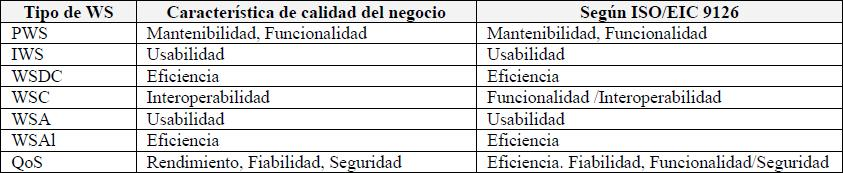
\includegraphics[width=0.9\textwidth]{CalidadSW}
  \caption{Características de Calidad asociadas al tipo de Servicio Web}
  \label{fig2:SW}
\end{figure}



\begin{quotation}
Para poder implementar un servicio Web se cuenta con las siguientes tecnologías:
\end{quotation}

\begin{itemize}\itemsep=0pt
\item  \textbf{Protocolo Simple de Acceso al Objeto (SOAP).-} Es un estándar de la World Wide Web Consortium (W3C) que describe un formato de mensaje (basado en XML) y mecanismos para intercambiar información entre aplicaciones, en un ambiente distribuido y descentralizado.
\item  \textbf{Lenguaje de Definición del servicio Web (WSDL).-} Es un estándar de la W3C que define un lenguaje basado en XML que permite describir la interfaz, formas de acceso y ubicación de un Servicio Web.
\item  \textbf{Universal Descripción, Descubrimiento e Integración (UDDI).-} Estándar de la
Advancing Open Standards for the Information Society (OASIS) que provee una forma estándar de publicar, categorizar y buscar Servicios Web.
\end{itemize}

\begin{quotation}
Debido a que en este proyecto el objetivo es que cualquier persona pueda subir una imagen de un cariotipo y mediante un procesamiento e interacción con un servicio Web se pueda obtener un reporte del cariotipo analizado se va a usar un Servicio Web para Análisis (WSA).\\
\end{quotation}

\begin{quotation}
Para lograr lo comentado, se procederá a realizar compresión de imágenes. Las imágenes se han convertido en un área muy importante de informática. Hoy en día surgen más entornos gráficos orientados a múltiples aplicaciones. El uso de las imágenes se ha incrementado con el desarrollo de la informática, de igual forma su resolución (y por tanto tamaño), de ahí la necesidad de compactarlas para reducir la cantidad de datos a enviar por la web. La compresión se basa en la eliminación de datos redundantes; dicho de otra forma, equivale a transformar una distribución bidimensional de pixeles en un conjunto de datos estadísticos sin correlacionar. Esta transformación (compresión) es aplicada a las imágenes antes de que sean almacenadas o antes de ser enviadas, por ejemplo vía red o internet. %\\
\end{quotation}

\begin{quotation}
Con la compresión de imágenes se trata de minimizar el número de bits para representar una imagen. Las aplicaciones de la compresión de imágenes son principalmente la transmisión y almacenamiento de información. En trasmisión, sus principales aplicaciones son la televisión, el radar, redes de computadoras entre otras. En almacenamiento, la compresión de imágenes se utiliza sobre documentos, imágenes de satélite, imágenes médicas. Debido a lo comentado es que se requiere un procedimiento para realizar la compresión para que se pueda enviar al Servicio Web de manera rápida y sin perdida de información y realizar el cariotipo. % \\
\end{quotation}


%%%%%%%%%%%%%%%%%%%%%%% PLANTEAMIENTO DEL PROBLEMA

\section{Planteamiento del Problema}\label{planteamientoproblema}


\begin{quotation}
Como se vio en el marco teórico (sección 4. Marco teórico), el análisis de cromosomas (cariotipo) de aproximadamente 12 horas de trabajo, debido a la falta de herramientas automáticas que simplifiquen esta tarea; en consecuencia la cantidad de cariotipos que pueden realizarse es baja. Si a esto se le añade el costo de microscopios especializados este análisis se vuelve prohibitivo para comunidades rurales o marginadas cuyos centros de salud poseen en el mejor de los casos microscopios con características básicas. Por ello, los pacientes se ven forzados a desplazarse a las ciudades cercanas (lo cual implica un alto costo de traslado, alimentación, etc.) para realizar dicho análisis.
\end{quotation}

\begin{quotation}
Para resolver esta problemática, se plantea desarrollar un servicio web que permita la transmisión de $n$ imágenes de cromosomas de una persona a través de Internet y regrese los resultados, todo mediante una página web. Dicha tarea no es sencilla, pues cada imagen es superior a los $500kb$ y considerando la velocidad de las comunicaciones en comunidades alejadas no es buena la eficiencia en dicha transmisión se convierte en una prioridad.
\end{quotation}

\begin{quotation}
Debido a los detalles mencionados anteriormente, se desarrollará un servicio Web para atender esta problemática donde se pretende cubrir los siguientes puntos:
\end{quotation}


\begin{itemize}  %\itemsep=0pt
\item  Integrar un Servicio Web disponible para cualquier Centro de Salud principalmente los ubicados en zonas rurales.
\item  Que las Instituciones y Centros de salud públicos puedan realizar el estudio de cariotipo sin tener que invertir cantidades elevadas de dinero en instrumentación especializada. Este estudio se podrá realizar solamente contando con un microscopio con características básicas en un precio entre 50,000 y 70,000.00 M.N.
\item  Establecer un proceso de empaquetamiento para la imagen del cariotipo, que permita poder transferir la imagen lo más rápido posible considerando zonas rurales donde la velocidad y los métodos para conectarse a internet dependan de dispositivos de baja velocidad de transmisión, por ejemplo un modem.
\end{itemize}


%%%%%% 


%%%%%%%%%%%%%%%%%%%%%%% HIPOTESIS

\section{Hipótesis}\label{hipotesis}

%\begin{quotation}
%Hipótesis
%\end{quotation}

\begin{quotation}
Debido que este tipo de análisis se realiza en ciudades grandes que cuentan con Instituciones y Centros de Salud de alta especialidad, pero que a su vez implica un mayor costo en los servicios que ofrecen al público en general, genera un costo considerable para las personas que viven en el campo ya que deben de realizar gastos de traslado y alimentación a las ciudades donde se encuentran estos centros de salud u hospitales que cuentan con este servicio de análisis cromosomático.
\end{quotation}

\begin{quotation}
El uso de herramientas web para el análisis de cromosomas permite reducir los costos del análisis tradicional al permitir realizar el análisis utilizando microscopios de bajo costo, por lo que es más accesible para la población acercarse a un centro comunitario de salud a tener que realizar traslados a una ciudad.
\end{quotation}


%%%%%%%%%%%%%%%%%%%%%%% OBJETIVOS

\section{Objetivos}\label{objetivos}

\begin{quotation}
Objetivo general
\end{quotation}
\begin{quotation}
Desarrollar e implementar un sistema computacional flexible que utilice un Servicio Web, amigable para el usuario, auxiliar en el diagnóstico de enfermedades genéticas, que sea capaz de generar cariotipos automáticamente aplicando algoritmos de procesamiento digital en imágenes obtenidas en procedimientos cito genéticos estándar y cuyos resultados de clasificación sean similares a los obtenidos por un experto.
\end{quotation}

\begin{quotation}
Objetivos específicos:
\end{quotation}

\begin{quotation}
\begin{itemize}\itemsep=0pt
\item Implementar un Servicio Web para el procesamiento de las imágenes que se utilizarán para el estudio del cariotipo.
\item Implementar un mecanismo de compresión de imágenes que permitan su facil transferencia al proceso de análisis de la misma.
\item Implantar el sistema propuesto en un centro hospitalario.
\end{itemize}
\end{quotation}

%%%%%%%%%%%%%JUSTIFICACION
\section{Justificación}\label{Justi}

\begin{quotation}
Debido a que las Instituciones y Centros de Salud públicos cuentan con recursos limitados para su operación, por lo tanto la adquisición de equipo para realizar el cariotipo (microscopio y el software para su operación) no resulta viable. Es por esta razón que muchos pacientes se ven obligados a recibir este servicio en centros de salud privados o en centros de salud en otras ciudades, que en ambos casos implica un costo que la mayoría de ellos no pueden solventar. 
\end{quotation}

\begin{quotation}
Es por esta razón que nuestra propuesta de tesis considera el desarrollo de una plataforma web que permita a distintos centros de salud pública realizar cariotipos (empleando microscopios con tecnología básica). 
\end{quotation}


%%%%%%%%%%%%% LIMITACIONES...
\section{Alcances y limitaciones}\label{limitaciones}

La presente propuesta de tesis se limitará a:

\begin{itemize}\itemsep=0pt
\item Proveer una herramienta web para cariotipo exclusivamente.
\item Proporcionar una herramienta que permita acelerar la transferencia de las imágenes mediante una técnica de compresión.
\item Proporcionar un Servicio Web que procese, reciba y descomprima las imágenes para finalmente elaborar un informe. Dicho informe servirá como una herramienta de apoyo al diagnóstico médico.
\item Para la generación del cariotipo se definirá un umbral mínimo de calidad de las imágenes de entrada (separación entre cromosomas y resolución).
\end{itemize}


%%%%%%%%%%%%%%%%%%%%%%% METODOLOGIA
\section{Metodología de Investigación}\label{metodo}

La metodología de investigación que se seguirá durante el desarrollo de la presente propuesta de tesis se divide en 2 etapas:

\begin{itemize}
\item Durante la primera se investigará acerca de los tipos de servicios web, las estrategias y el software requerido existentes para su implementación. En este punto se revisarán las arquitecturas existentes para SOAP y REST. Así mismo, durante el desarrollo de esta etapa se montará un servidor local para realizar la implementación y las pruebas. Para ello se revisará la tecnología Linux ya que es de uso libre. Finalmente se iniciará con la investigación de las técnicas de compresión de imágenes existentes que permitirá agilizar la transferencia de imágenes entre el cliente y el servicio web.\\

\item En la segunda etapa del proyecto se investigará sobre los métodos de compresión de imágenes, primeramente analizando los diversos métodos  existentes en la actualidad para determinar el método más adecuado que nos permita realizar una compresión de calidad y que ocupa pocos bytes de espacio. Una vez terminada la compresión de imágenes se procederá a integrarlo con el servicio web para empezar a realizar las pruebas de la aplicación de cariotipo. En este punto podemos empezar a elaborar el manual para el usuario pueda realizar el cariotipo con este proyecto para finalmente implantar el sistema en el HIT.\\

\end{itemize}


%%%%%%%%%%%%%%%%%%%%%%% CRONOGRAMA

\section{Cronograma de Actividades}\label{cronograma}
%\begin{quotation}
%Cronograma de Actividades
%\end{quotation}



\begin{center}
%\begin{sideways}
\scalebox{0.75}{
\begin{tabular}{|l|c|c|c|c|c|c|}
\hline
\textbf{\centering Actividad} & \textbf{Bim-I} & \textbf{Bim-II} & \textbf{Bim-III} & \textbf{Bim-IV} & \textbf{Bim-V} & \textbf{Bim-VI} \\
\hline
Investigar Estado del Arte (Cariotipado) & \cellcolor{black} & \cellcolor{black} &   &   &   &  \\ 
\hline
Investigación sobre Servicios Web &  & \cellcolor{black} &  \cellcolor{black}  &   &   &  \\
\hline
Inv. Métodos de Compresión de Imágenes & \cellcolor{black} &  \cellcolor{black} &  &  &  &  \\
\hline
Implementación del WebService &   &  & \cellcolor{black} &    &    &  \\
\hline
Implementación del Métodos de Compresión &   &   & \cellcolor{black} &   &   &  \\
\hline
Diseño e implementación de interfaz &   &   &  & \cellcolor{black} & \cellcolor{black} &  \\
\hline
Pruebas &   &   &  \cellcolor{black}  & \cellcolor{black} &  & \\
\hline
Artículo &   &   &   &  \cellcolor{black}  & \cellcolor{black}  &  \\
\hline
Reporte de Beca &   & \cellcolor{black}  & \cellcolor{black}  &  \cellcolor{black}   & \cellcolor{black} & \cellcolor{black} \\
\hline
Tésis &   & \cellcolor{black} &   & \cellcolor{black}  &   &   \cellcolor{black} \\
\hline
Defensa del exámen &   &   &   &  &   &  \cellcolor{black}\\
\hline
\end{tabular}}
%\end{sideways}
\end{center}



\newpage
\bibliographystyle{abbrv}
%\bibliographystyle{unsrt}
%\bibliographystyle{apalike}
\bibliography{bibliografia}


\end{document}

